% !TeX spellcheck = en_US
\renewenvironment{longtable}{\rowcolors{2}{LightGray}{white}\oldlongtable} {\endoldlongtable}
\chapter{基本串口应用——\acs{USART}}

串口是一种非常古老的机器间串行通信方式,它可以支持异步全双工通信,也就是说不需要同步时钟信号,而且可以同时双向传输数据。因此,串口的接线方式也非常简单,在大多数应用场景下,只需要4根信号线(一对电源,一对数据线)甚至3根信号线(电源可以只提供参考地电平)即可连接。而它的传输速率也具有很高的灵活性,每秒传输的二进制位数(即波特率,baudrate)可以选取4800、9600、38400,甚至115200以及更高。这些特性使串口在单片机应用中成为一种流行的通信方式,例如大多数GPS模块都默认以串口方式传输数据。此外,串口也可以与我们的计算机相连,由单片机向计算机打印调试数据,或者由计算机向单片机发送控制命令,极大地方便了我们的调试工作。因此,我们在这一章对串口编程进行介绍,之后的章节中,就可以利用串口直接打印实验结果,而不需要深入介绍其他显示设备——事实上,在飞行控制中,大多数情况下也不需要安装液晶屏等显示设备,而可以直接利用串口调试。

\section{串口的工作机理}
\subsection{串口的连接方式}
要实现基本的数据传输功能,串口只需要4根连接线,如下表所示。
\begin{center}
	\begin{longtable}[c]{| l | l |}
		\caption{串口接线}	\label{chart:usartWire}\\
		\hline 
		\rowcolor{Gray}
		\textbf{名称} & \textbf{描述} \\
		\hline
		\endfirsthead
		
		\hline 
		\rowcolor{Gray}
		\textbf{名称} & \textbf{描述} \\
		\hline
		\endhead
		
		Vcc & 电源线\\
		GND & 参考地电平\\
		Rx & 数据接收线,连接另一设备的Tx\\
		Tx & 数据发送线,连接另一设备的Rx\\
		
		\hline
	\end{longtable}
\end{center}
\newpage
当然,完整的串口定义还包含一些其他的控制线,但在大多数场景中上述的4条接线已经足够了。

\subsection{串口的信号时序}
如果我们配置串口的通信模式为8位数据,1位停止位,无校验位,那么它的通信时序如图\ref{fig:usartTime}所示\footnote{截自\acs{RM}}。
\begin{figure}[h]
	\begin{center}
		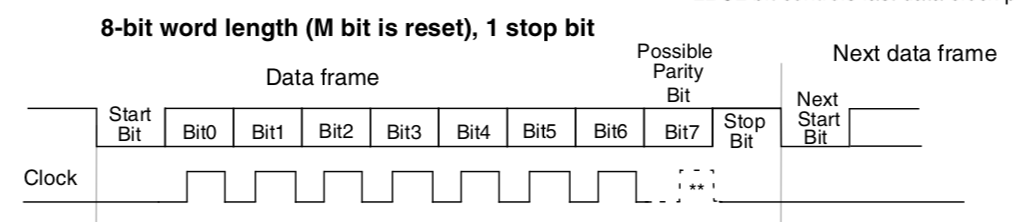
\includegraphics[width=0.85\textwidth]{images/content/usartTime.png}
		\captionof{figure}{串口信号时序}
		\label{fig:usartTime}
	\end{center}
\end{figure}
\par 
其中的时钟信号(Clock)在实际连线中并不需要,这里画出只是作为参考。
\par 
可以看到,串口数据传输一般以字节为单位,传输开始时信号线被拉低一个时钟周期作为起始标志。接收方收到起始位之后需要按约定好的波特率同步自身的时钟,以正确进行当前字节的接收。之后的8个时钟周期依次传输字节的8个二进制位,最后一个周期拉高信号线作为停止标志。如此周而复始,不断地传输数据。容易发现,由于每个字节都有起始位作为同步信号,而且传输的波特率一般不会很高,这使得没有时钟线的异步通信方式对时钟的误差不会累积,也不会很敏感。当然,这也限制了串口通信的速率。

\section{STM32的串口支持}


















